\documentclass[12pt]{article}
\usepackage[utf8]{inputenc}
\usepackage{amsmath}
\usepackage{amssymb}
\usepackage{amsthm}
\usepackage{enumitem}
\usepackage{mathtools}
\usepackage{lipsum}
\usepackage{mwe}
\usepackage[letterpaper]{geometry}
\geometry{margin=0.8in}
\usepackage{hyperref}
\usepackage{xcolor}
\usepackage{listings}
\usepackage{xparse}
\usepackage{url}
\usepackage{sectsty}
\sectionfont{\LARGE}
\NewDocumentCommand{\codeword}{v}{%
\texttt{\textcolor{blue}{#1}}%
}



% The title of the report
\title{
\vspace{80}
\begin{figure}[h]
  \centering
    
\includegraphics[scale=2]{figures/mcgill_sig_red.jpg}
\end{figure}
\vspace{50}
Frame Prediction of Aerial Objects
\vspace{20}

COMP 558 Project Report
\vspace{50}
}
% Authors
\author{Jonathan Lane-Smith, Rongge Zhang, Keyu Wang \vspace{30}}
% Course code and date
\date{December 15, 2022}

\begin{document}

\maketitle
\clearpage

\section*{Abstract}

Next frame video prediction is an active research topic with extensive applications in many areas, such as autonomous driving and robotic decision-making. Recent developments in deep learning have allowed for the prediction of future events by analyzing historical frame data. In this project, we focused on predicting the paths of aerial objects using a stationary camera and classical computer vision algorithms. We implemented a sequence of methods including Farneback optical flow, Meanshift object tracking, RANSAC with least squares, Canny edge detection and median filtering for background generation. To demonstrate our results, we will present an example of a recorded video with the predicted frames added to the end. We found that the classical computer vision algorithms were effective for detecting the object, tracking it, predicting its path, copying it, and pasting it onto future frames. However, our implementation of these algorithms was not very robust and would only work with particular videos in which the object is very distinct from the background. Furthermore, our algorithms made a number of assumptions about the object, such as no rotation or movement along the z-axis. Nevertheless, given the assumptions we made, we were successful at predicting future frames, proving that classical computer vision algorithms are useful and effective for frame prediction.

Keywords: frame prediction, video sequence, Farneback optical flow, object tracking, RANSAC, object extraction, background modelling.


\section*{Background}
Frame prediction involves determining the location of an object in the next frame of a video or image sequence. If the moving object can be accurately identified, object tracking becomes a series of matching problems based on the position, speed, shape, texture, colour, and other relevant feature information between successive frames. When the object is tracked successfully, we have information about its motion between frames, which allows us to predict its location in future frames. Therefore, the key challenges of frame prediction include moving object detection, object tracking, and trajectory prediction.

\subsection*{Object Detection}
When detecting an object, the background can either be static or dynamic, depending on the relative motion between the object and the camera. Eliminating the movement of a background is a complex problem, and for this project, we will only consider the static background case. The goal of moving object detection in a static background is to identify and separate the moving object from the background in a video or image sequence. This can be done using several methods, such as the background difference method, the frame difference method, and the optical flow method.

Background difference: \cite{stauffer1999adaptive} divides the image into background and foreground, models the background, and then uses the difference between the current frame and the background image to detect the moving area. This method can obtain more accurate moving object information, but it is especially sensitive to the dynamic changes in a scene, such as illumination and interference from external unrelated events.

Frame difference: In a continuous image sequence of adjacent frames, the pixel-by-pixel differences are used to find the changing areas in the image, which may correspond to the moving areas in the image \cite{meier1999video}. However, it may misjudge the moving object, and the frame difference method is not as effective if the object is moving slowly.

Optical flow: This method involves calculating the optical flow vector for each pixel in the image, which allows the motion field of the image to be determined. If there is a moving object in the image, the optical flow of the moving object will be significantly different from the motion vector of the  background. Through this method, the moving object in the image can be detected.

\subsection*{Object Tracking}
To track an object in a video, information about the object, such as its size, shape, and pixels, is used. In each frame of the video sequence, the region that is most similar to the object is found, which allows the position of the object to be determined. After researching the object tracking algorithms based on classical computer vision methods, we conclude that they can be generally divided into three categories: points feature and optical flow based tracking, region kernel function based tracking and contour model based tracking.

Points feature and optical flow based tracking: In \cite{4522480}, Harris corner detection is combined with the optical flow method, and the pixels in the optical flow method are replaced by Harris feature points for object tracking. This reduces the number of tracking pixels, which reduces the complexity of the algorithm and speeds up the processing speed. \cite{rodriguez2012real} put forward the concept of artificial optical flow, in which the real optical flow can be compared with the artificial optical flow by vector differences in object movement. However, object tracking based on optical flow has many disadvantages. It calculates all the pixels in the video and has poor performance for real-time tracking.

Region kernel function based tracking: The kernel function tracking method is used to track the motion of an object in a video by comparing the area occupied by the object in two consecutive frames. This method calculates the motion of the object's region and finds the most similar area in the next frame by comparing the similarities between the motion areas. The MeanShift algorithm \cite{comaniciu2002mean} is a typical kernel tracking method that matches in the direction of an increasing probability density function. This algorithm can quickly find the position that is most similar to the object with fewer iterations than other methods. Based on it, many other improved algorithms have been put forward, such as the CAMShift algorithm \cite{nouar2006improved}.

Contour model based tracking: For tracking a rigid object, a 3D model of the object can be built. Then, the parameters of the 3D model can be determined according to the actual image and one can determine the motion parameters of the object. The disadvantage of this method is that the accuracy of motion analysis depends on the accuracy of geometric models, and it is very difficult to obtain accurate geometric models of all moving targets in a real application. This limits the use of model-based tracking algorithms. In \cite{hu2004survey}, the author gives a detailed introduction to the model-based tracking algorithm.

\subsection*{Trajectory Prediction}
To determine the position of a moving object in the next frame, its trajectory can be predicted using object tracking. The trajectory of an object can be thought of as a series of points that change over time. There is usually a pattern to these changes, which can be used to predict the object's future trajectory. The most common methods for predicting an object's trajectory are polynomial fitting and the Kalman filter.

Polynomial fitting: The trajectory of an object can be approximated by fitting a polynomial to the known trajectory points and time. This allows the spatial position of the object to be predicted for a given moment. As the most traditional trajectory prediction method, polynomial fitting has the advantages of a simple principle, easy implementation, and fast modelling. It is effective for simple trajectory predictions with a small amount of data.

Kalman filter: In the trajectory prediction of moving objects, the Kalman filter algorithm estimates the state of the object's behaviour, then updates the estimation of state variables using the estimated value from the previous moment and the observed value of the current moment, and finally predicts the trajectory position of the next moment. The main shortcomings of the Kalman filter algorithm are that it cannot make accurate long-term predictions and does not perform well when the system model and the statistical characteristics of noise are not clear.

\subsection*{An Overview of Deep Learning-based Object Tracking and Prediction}
Deep learning is a rapidly developing technology that has been applied successfully in the field of frame prediction. Deep learning is not intended for our project, but it will be briefly covered here.
We focus on the 2022 IEEE/CVF Conference on Computer Vision and Pattern Recognition, and there are quite a few related papers accepted. Many papers are based on transformers, including \cite{mayer2022transforming} \cite{cao2022tctrack} \cite{Zhou2022GlobalTT}. There are also some other papers that use a diffusion model \cite{gu2022stochastic},  graph neural network (GNN) \cite{xu2022adaptive} and causal representation \cite{liu2022towards}. These papers represent the state-of-the-art technology in frame prediction, showing excellent performance, but also requiring a heavy computing complexity.

Moving object detection, tracking, and trajectory prediction are important research areas in the field of computer vision. Many effective algorithms have been developed to address these challenges. However, the goal of achieving robustness, accuracy, and real-time performance in frame prediction algorithms has not yet been fully achieved and continues to be pursued.


\section*{Methods}

In order to successfully implement frame prediction, there were 6 main steps. First, we needed to find the location of the object in the image. Second, we needed to track the movement of the image throughout the frames. Third, using this information, we needed to model its movement and predict a future path. Fourth, we needed to retrieve the shape of the object so that we can "copy and paste" it onto future frames. Fifth, we needed to extract the background so that we can remove the object from the frame, before pasting it back in. Finally, we pasted the object onto its predicted locations to generate the predicted frames.

\subsection*{Object Detection}

We chose to detect the object by finding the maximum optical flow magnitude in the image. However, when an aerial object is at its vertical peak, it may be moving very slowly. The easiest way to detect a moving object using optical flow is when it is moving quickly. Therefore, we chose to search through the whole video, to find the frame when the object is moving the fastest.

To detect the moving object, we initially chose to use the Lucas-Kanade optical flow algorithm. For each video frame, we calculated the optical flow in the image and found the pixel with the greatest magnitude of optical flow, meaning it is moving the fastest. We then searched through each frame, to find the frame which had the fastest pixel. This corresponded to the fastest-moving pixel during the whole video, which we assumed to be the aerial object.

Unfortunately, this technique had a number of issues. The Lucas-Kanade optical flow algorithm incorrectly categorized some non-moving pixels in the image as moving very quickly, which prevented the algorithm from accurately detecting the object. To address this issue, we chose to implement Farneback optical flow. Farneback optical flow, invented by Gunnar Farnebäck, uses quadratic polynomials to estimate displacement fields and this results in a more robust algorithm \cite{farneback2003}. By using Farneback optical flow, the optical flow became less error-prone, which made the algorithm more reliable.

However, the program would still sometimes choose pixels that did not belong to the moving object. To address this problem, we implemented a small algorithm to ignore these pixels. Because the overall speed of the aerial object changes relatively slowly, the maximum optical flow magnitude should be fairly similar between each frame, if the program is truly tracking the object. When comparing the maximum optical flow magnitude between frames, if the difference between these values is above a certain threshold, then we can assume that the pixel being tracked does not belong to the object. After experimenting with different thresholds, we were able to implement this algorithm and this solved the problem, allowing the object to be correctly detected.

Finally, we noticed that the estimated "point" of the object was not in the middle of the object, as we desired it to be. To solve this, we added code that, after finding the point of maximum optical flow, searches the local neighbourhood of that point to calculate the average position of the optical flow, using a weighted sum algorithm. The object's true center was much closer to the average flow position than to the point of maximum flow.


\subsection*{Object Tracking}
To track the motion of an object in a sequence of frames, we start by identifying the frame with the maximum optical flow. We then go backwards in time, tracking the object and recording its position. In this process, the frame with the earlier timestamp is treated as the next frame to track. We also track future frames and record the object's position in these frames too. To track the object, we first select an interest region in the object's vicinity and use the Meanshift algorithm. We found that the size of the interest region can affect the tracking performance.

To use the Meanshift algorithm, we first calculate the colour histogram distribution of the rectangle box in the selected tracking area. We then calculate the histogram distribution of the corresponding rectangle box in the next frame and use these distributions to calculate the Meanshift vector, which represents the movement of the object between frames. The search window is then moved in the direction of the highest probability density. By repeating this process for each pair of frames, we can continually update the coordinate position of the object's center point as it is moving.

The Meanshift vector is defined as the vector sum between $t$ sample points and the geometric center of the region, where  ${x_i}$ is the sample point and  $x$ is the geometric center of the region. ${S_h}$  is the sphere region with radius $r$  conforming to the calculation region.
\[{M_h}(x) = \frac{1}{t}\sum\limits_{{x_i} \in {S_h}} {({x_i} - x)} \]

\[{S_h}(x) = \{ y:{(y - x)^T}(y - x) \le {r^2}\} \] 

The direction of the vector sum is the direction of increasing probability density. To find the optimal solution, we move the vector along this direction and iterate gradually. The probability density is determined by the similarity of colour and spatial proximity between the target pixel and sample pixels. The higher the similarity and proximity, the higher the probability density. A diagram of the Meanshift tracking principle is shown in Figure \ref{Meanshift schematic}.
\begin{figure}[h]
  \centering
    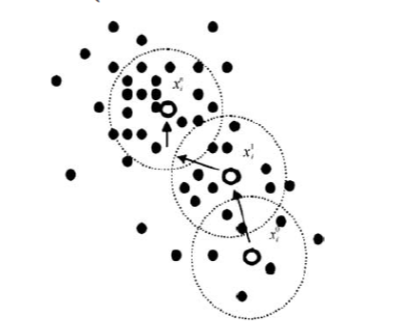
\includegraphics[scale=1]{figures/meanshift.png}
    \caption{The tracking schematic of Meanshift}
    \label{Meanshift schematic}
\end{figure}

The Meanshift algorithm has 5 main steps, as shown below.

1)	Calculate the object model.
Suppose the dimension of the histogram is $m$. The number of pixels is $n$, the center of the object is  ${x_0}$, and the radius is $h$. There is a one-to-one mapping function $b({x_i})$ between the pixel value of each pixel and the colour histogram. The probability density of the feature of the object model is:\[{q_u} = C\sum\limits_{i = 1}^n {k[{{\left\| {\frac{{{x_0} - {x_i}}}{h}} \right\|}^2}]} \delta [b({x_i}) - u] \]
In this equation, $k$ represents the kernel function, $\delta$ represents the Kronecker function, and $C$ represents the normalization coefficient.

2) From the current frame, select the candidate object’s initial position $y$. For each following frame, suppose $\{ {x_i},{x_i} = ({x_i},{y_i})\}, i = 1,2, \cdots {n_h}$ is the candidate pixel position of the object in the frame and $y$ is the center position of the object, so the probability density function of the colour $u \in \{ 1, \cdots ,m\} $ in the candidate object is:\[{p_u}(y) = {C_h}\sum\limits_{i = 1}^{{n_h}} {k[{{\left\| {\frac{{y - {x_i}}}{h}} \right\|}^2}]} \delta [b({x_i} - u)]\]

3) Calculate the similarity between the target model and the candidate model.
\[\rho  = \sum\nolimits_{u = 1}^m {\sqrt {{p_u}(y){q_u}} } \]
The more similar the target model is to the candidate model, the larger $\rho $ is.

4) Calculate the offset position of the object in the current frame, where the center moves from  ${y_0}$ to the new position ${y_1}$:
\[{y_1} = \frac{{\sum\limits_{i = 1}^{{n_k}} {{x_i}{w_i}g({{\left\| {\frac{{{y_0} - {x_i}}}{h}} \right\|}^2})} }}{{\sum\limits_{i = 1}^{{n_k}} {{w_i}g({{\left\| {\frac{{{y_0} - {x_i}}}{h}} \right\|}^2})} }}\]
In the above equation, ${w_i}$ is defined as \[{w_i} = \sum\nolimits_{u = 1}^m {\sqrt {\frac{{{q_u}}}{{{p_u}(y)}}} } \delta [b({x_i}) - u]\]

5) Calculate the probability density of the candidate model at the new position ${y_1}$, and calculate the similarity between the new candidate target and the target template. If $\left| {{y_1} - {y_0}} \right| < \varepsilon $, the optimal position ${y_1}$ is found. Otherwise, set ${y_1}$ to ${y_0}$ and turn to 2) to start the iteration again.

For this part, we referred to some blog examples for the calculation of the Meanshift vector and similarity coefficient\cite{meanshiftblog1}\cite{meanshiftblog2}. We implemented the colour histogram, the position update, and the forward/backward tracking process by ourselves.


\subsection*{Path prediction}

Since aerial objects are only acted upon by gravity, we decided to fit the object's center coordinates to a parabola using least squares. However, sometimes the tracked object path would have sequences where the points were not tracking the object correctly. Therefore, we chose to combat this by implementing RANSAC. We set the total number of trials to be 200 times the total number of points, and the maximum allowable distance for a point to be an inlier half of the object length.

After fitting the curve, we plotted the future object coordinates for each frame using the same gap between x-values to generate their corresponding y-values. This is because horizontal velocity for a parabolic motion is constant when there is minimal air resistance or wind. This assumption was safe to make because our videos were all shot indoors.
\begin{figure}[h]
  \centering
    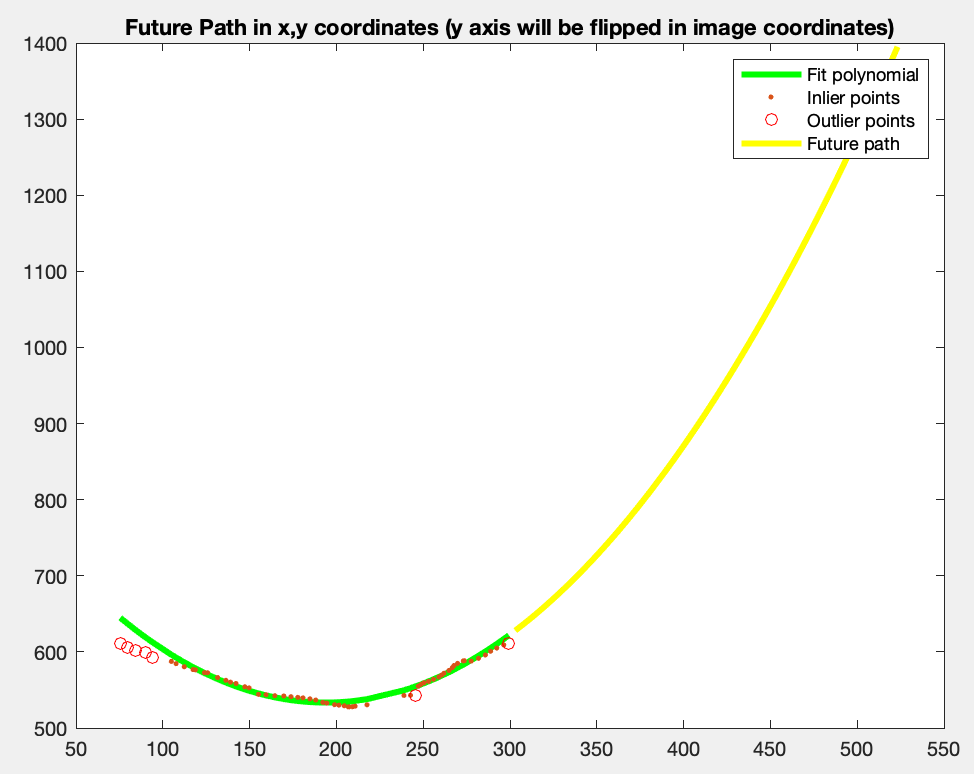
\includegraphics[scale=0.4]{figures/ransac1.png}
    \caption{Path prediction in flipped image coordinates using RANSAC}
    \label{RANSAC results}
\end{figure}


\subsection*{Object Shape Retrieval}

In order to predict future frames, we needed to "copy" and "paste" the moving object to its predicted locations. We implemented two different methods to copy the image.

The first method runs the Canny edge detector on the frame indicated by the object detection algorithm. This frame contains the object when it is moving at its fastest. The algorithm then removes any edges for which its optical flow (calculated using the Farneback algorithm) is not above an experimentally determined threshold. The purpose of this is to remove edges which are not moving, which makes it easier to identify the moving object.

After this, we assume that there is a solid line that fully surrounds the object. Presuming that the point provided by the object detection algorithm is within the bounds of the shape, we start from that point and recursively spread out, in order to "fill in" the shape. Doing this will cause all pixels in the shape to have a value of 1, instead of just the edge pixels. This recursive algorithm also allows the height and width of the object to be found.

Following this, we wrote code to crop the edge detector output to the size and location of the image. This provides a "mask" which allows for just the pixels of the moving object to be pasted during the frame prediction process, instead of the whole rectangle surrounding the moving object.

When testing this out on the video in which an AirPods case is thrown, we noticed that there was some light which reflected off the case. The Canny edge detector considered this to be an edge, causing there to be a circle inside of the shape which separated the inner pixels from the aforementioned "filling" algorithm. In order for these inner pixels to also be filled in, another algorithm was implemented. For each row, this algorithm moves two pointers from each end towards the middle, and when it determines that the pointers are inside the shape, it fills in any pixels which are not yet filled in. This algorithm assumes that the moving object is convex.

This first method worked very well on the AirPods case in the first video we tested, but the other videos we tested had issues with this method. Most notably, the objects in the other videos did not have solid lines surrounding the objects, which made it impossible to "fill in" the objects. However, in these other videos, all of the moving objects were circular balls, and this assumption was used to form a second method.

In the second method, we start at the estimated shape center and use a side length of 1. Gradually increasing the side length, we sum up all of the edge pixels in a square centred at the estimated shape center. Once the sum of the edge pixels remains the same, we know that we have gotten to the boundaries of the shape. At this point, we crop the square to just be the moving object by removing any outer rows/columns without edges. This provides us with the radius of the object and we can then create a circular "mask" of those dimensions, to allow the object to be pasted onto future images.


\subsection*{Background Extraction}

Our background extraction method consists of 2 steps: first, we extract the pure static background, and second, we replace the object pixels from the last recorded frame with the extracted background so that the other moving objects of the last frame freeze instead of disappearing.

There are many methods for doing background extraction from a video that has minimal background shift. Ridder et al. \cite{Ridder1995AdaptiveBE} used foreground detection using a Kalman filter. Bailo et al. \cite{bailo2005} used background estimation with Gaussian distribution for image
segmentation and Shi et al. \cite{shi2002adaptive} introduced the adaptive median filter for background generation.

In this study, the mean/median filter method was
used because it is accurate for our case where we have a stationary camera posture and need the original colours. The equation used in the algorithm is the following\cite{rad2010vehicle}:

$$
k_{x y}\left(t_n\right)=\frac{\sum_{m=0}^{j-1} f_{x y}\left(t_{n-m}\right)}{j}
$$
In this equation: $\mathrm{n}$ is frame number; $f_{x y}\left(t_n\right)$ is the pixel value of $(\mathrm{x}, \mathrm{y})$ in n'th frame; $k_{x y}\left(t_n\right)$ is the pixel mean value of $(\mathrm{x}, \mathrm{y})$ in n'th frame averaged over the previous $j$ frames, and $j$ is the number of the frames used to calculate the average of the pixels value.

We built the method in a function called \codeword{getPureBackGrnd(filename, nTest, method)}. The function assumes 3 inputs, but when there are not enough inputs, we set the default number of frames to be tested = 20 and the default method to be "median". There is no need to use the entire clip to get the background image. The comparison between mean and median methods and the different numbers of frames used is illustrated below, which explains why we chose the default parameter values as described above.

\begin{figure}[h]
  \centering
    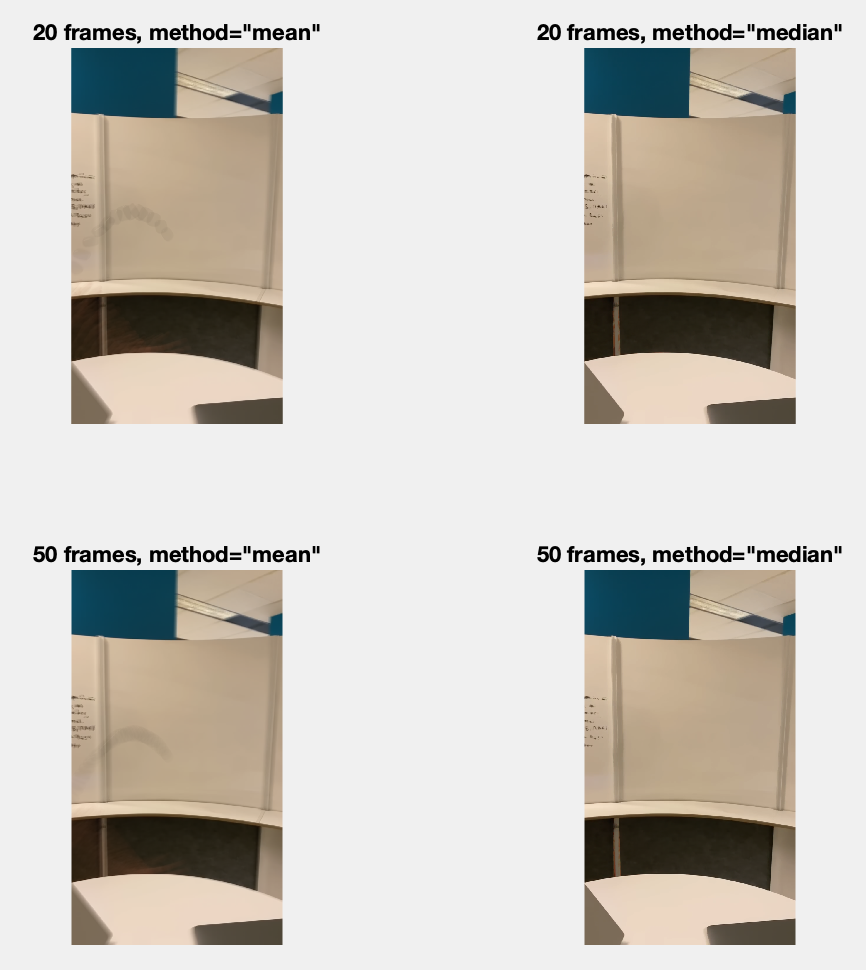
\includegraphics[scale=0.8]{figures/comparison_bg.png}
    \caption{Comparison between the pure background images extracted, using different numbers of frames and methods.}
    \label{Background Comparison}
\end{figure}

We can see from Figure \ref{Background Comparison} that the "median" method gives better results here, and there is not much difference as the number of frames used increases.

In addition to this, we also maintained a buffer of $B$ frames for dynamic estimation of the background, since if $f_i < B$ (i.e., processed less than B frames) the background model is not stable. We used NaNs as default values for the buffer, and the values will be ignored when the background model is estimated. Therefore we did not simply use \codeword{median} and \codeword{mean}, but \codeword{nanmedian} and \codeword{nanmean}.

We initially directly used the pure extracted background for the future frames, but we noticed that the other moving objects (that move at a slower speed than the main aerial object) would be erased from the background. In our AirPods case video, Jonathan's hand was erased from the pure background, which meant his hand would disappear when moving from the recorded footage to the predicted frames. Hence, we added step 2 to this part which is to "cut" the pixels from the pure background onto the last frame so only the detected aerial object will disappear from the background image.


\begin{figure}[h]
    \centering
    \begin{minipage}{0.5\textwidth}
        \centering
        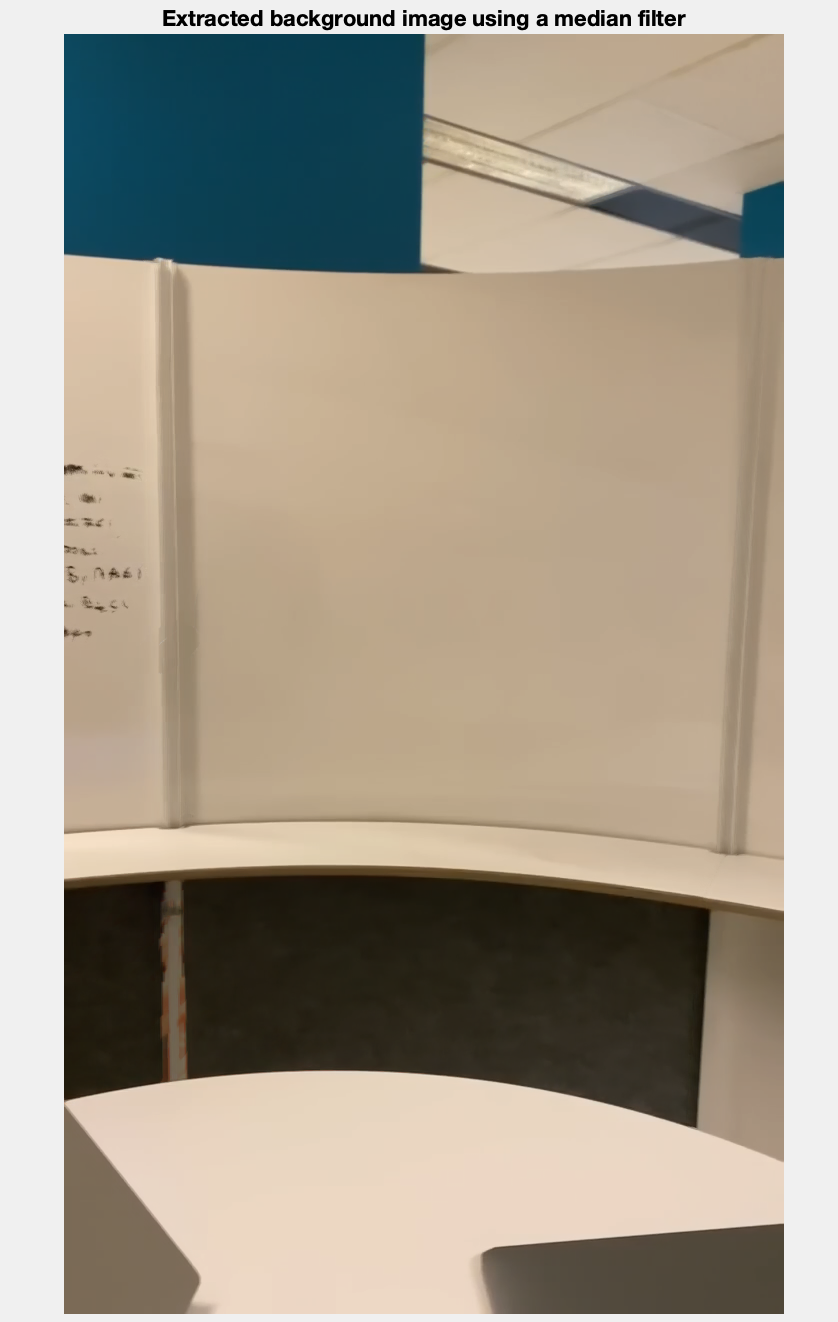
\includegraphics[width=0.9\textwidth]{figures/purebackground1.png}
        \caption{Pure background}
    \end{minipage}\hfill
    \begin{minipage}{0.45\textwidth}
        \centering
        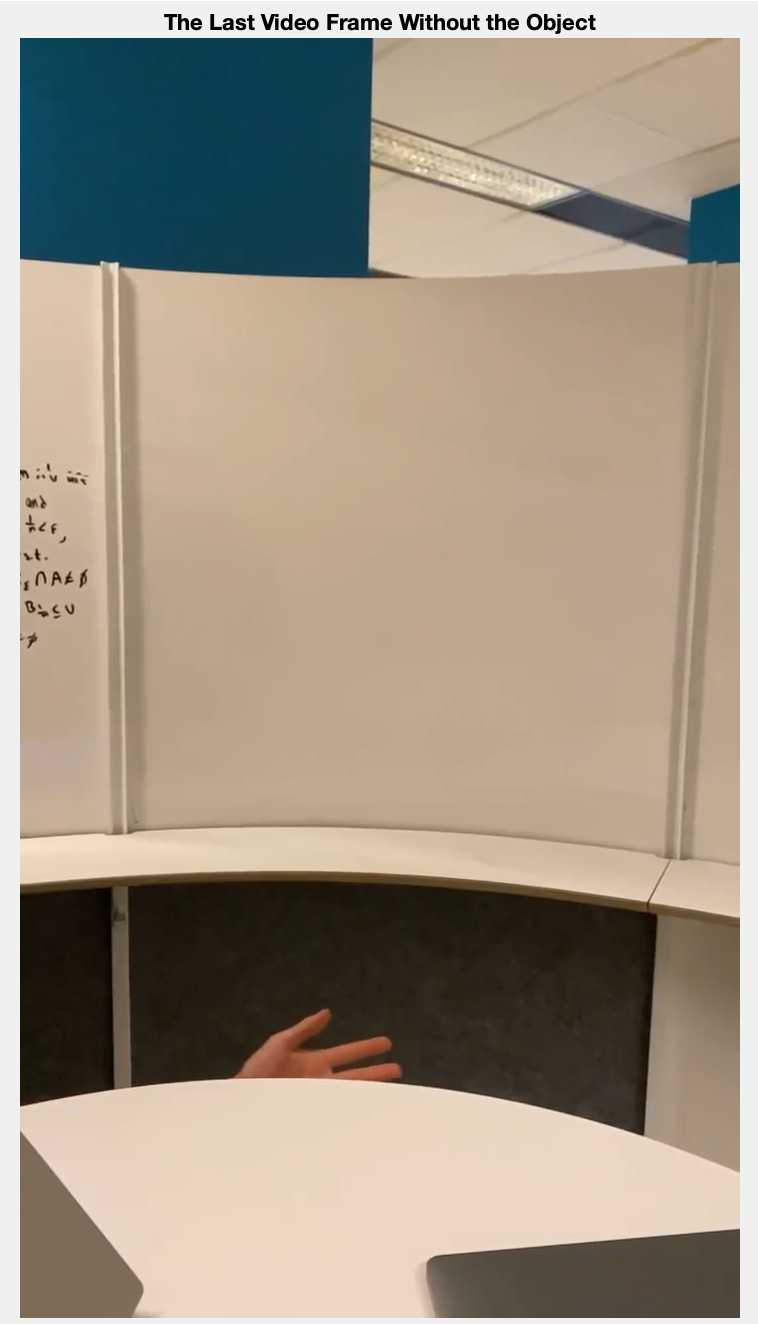
\includegraphics[width=0.9\textwidth]{figures/bg1.png}
        \caption{Last frame with the object erased}
    \end{minipage}
\end{figure}
\clearpage

\subsection*{Frame prediction}
At this point, we had the location of the object, a prediction of its trajectory, a background frame without the object, and the shape of the object. The next step was to predict the future frames of the object. We decided to show our results in 2 ways: one as an image that shows the path, and one as a video.

First, we pasted the object onto the image at its predicted location every 5 frames. We did this by simply replacing the image pixels from the background image with the object pixels. In the beginning, the spaces between the objects are quite small, and near the end, the object is moving faster so the spaces between the objects are larger. This image can be seen in Figure \ref{Object trajectory prediction} in the Results section of the report.

Next, we generated the video. The first part of the video consists of the actual recorded footage. The second part consists of the predicted frames. These predicted frames were made by taking the last frame of recorded footage, removing the aerial object, and pasting it onto the frame at its predicted locations for every frame. The video was created by generating frame-by-frame images as JPGs and then using MATLAB's \codeword{VideoWriter} and \codeword{VideoReader} to make sure that the frame rates match. When viewed in its entirety, the video shows the object being thrown and then continuing to move, even after the actual recorded footage has finished.



\section*{Results}

Overall, we were able to implement all 6 steps of our project and successfully predict the future frames of an object. Figure \ref{full path} shows the path tracking result after using Farneback and Meanshift, while Figure \ref{Object trajectory prediction} shows the predicted movement of the AirPods case, based on the previous frames. The actual video, consisting of the initial recorded frames and the generated predicted frames, is included in this project submission.


\begin{figure}[h]
  \centering
    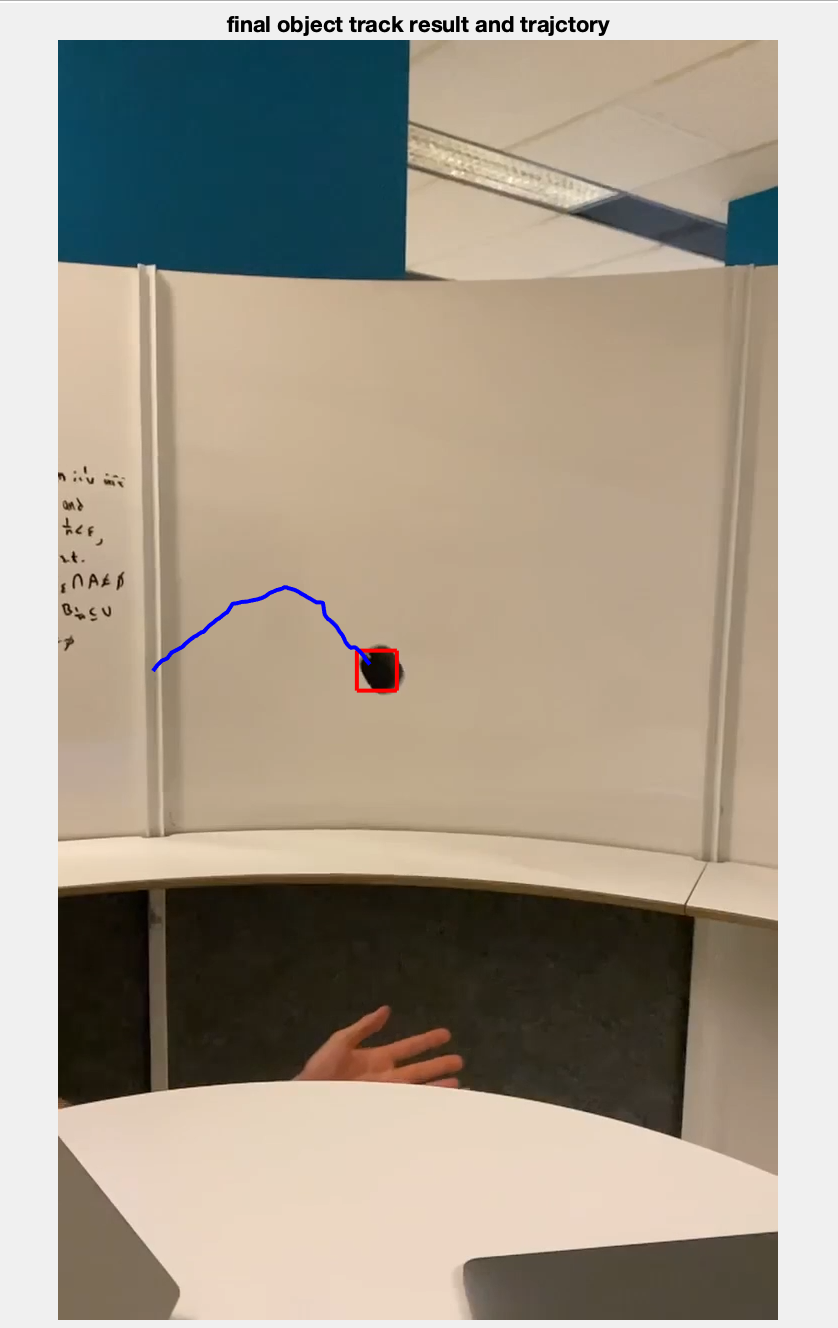
\includegraphics[scale=0.4]{figures/full1.png}
    \caption{Full path tracking result from Farneback and Meanshift}
    \label{full path}
\end{figure}

\begin{figure}[h]
  \centering
    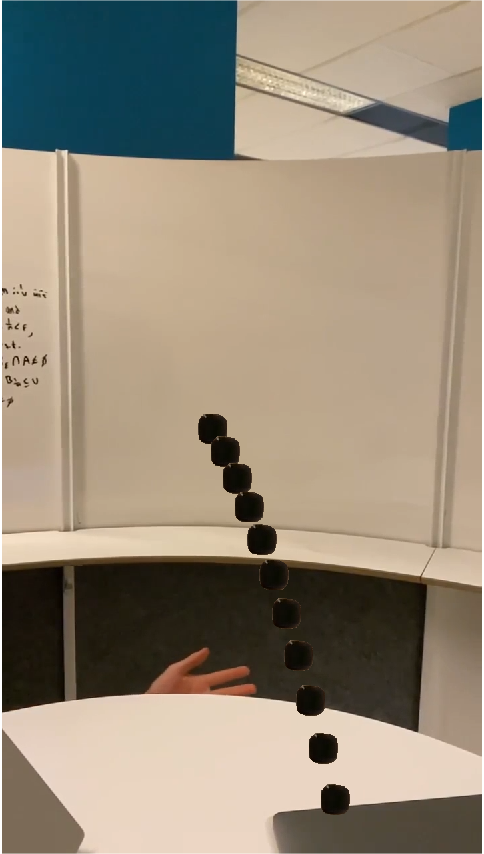
\includegraphics[scale=0.5]{figures/object_trajectory_prediction.png}
    \caption{Object trajectory prediction}
    \label{Object trajectory prediction}
\end{figure}

Unfortunately, we were not able to successfully implement this process for other videos. The other videos we tested our program on had less contrast between the moving objects and the backgrounds, and the moving objects had multiple colours and textures. This made it difficult to accurately track the object and retrieve its shape. Given more time, we could have refined our methods to make them more robust and flexible. With these refined methods, we would have been able to predict frames for more complicated objects of different shapes, sizes, colours, and textures.

\clearpage
\section*{Discussion}

This project combined a number of various computer vision algorithms. Optical flow, edge detection, modelling using least squares and RANSAC, and object tracking were all implemented in this project. Due to its complexity, there were many challenges and issues that arose. We were able to solve these issues by tweaking the algorithms to work for a specific video. However, this was not a robust solution that solved the issues for multiple different videos.

As mentioned in the Results section, the other videos had moving objects with more complexity and less contrast against the background. The second method for object shape retrieval (which assumes a circular shape and iteratively increases the size until the boundaries of the shape are found) gave acceptable results for some of these videos but not all of them. If the images had complicated backgrounds, the Canny edge detector would pick up on lines in the background, and this made it difficult to correctly find the shape of the object. The object shape retrieval algorithm would continue to increase the estimated object size as it searched for the boundaries of the shape, eventually reaching the boundaries of the full image.

Another disadvantage of our program was that it required a number of manual parameters before it could run. For each video, we had to specify which method it would use for retrieving the shape of the object (either method 1, which requires a solid line around the object, or method 2, which assumes a circular shape). We also had to specify the size of the interest region around the object. This interest region was used by the Meanshift tracking algorithm. If we were to continue working on this project, we could remove the need for this manual parameter by running the object shape retrieval algorithm before the object tracking. By finding the size of the object, we could use this to get an appropriate size for the interest region for object tracking.

Even if we were able to solve these issues and make our algorithms robust to videos with different objects, there are still a number of assumptions and constraints for our project. As mentioned earlier, we are assuming a static background, so videos with dynamic backgrounds would not work properly. We are also assuming one main moving object. If there were two moving objects, this might confuse the algorithms and they might come up with incorrect results. Furthermore, we are assuming that the moving object is small and convex. Irregularly-shaped objects might not be correctly tracked by our program. The object shape retrieval algorithms assume that the shape either has a solid line around it, or is circular.

We are also making a number of assumptions about the motion of the object. Specifically, we are assuming that the object is only being acted upon by gravity, that it has no rotation, and that it remains in the XY plane, without moving towards or away from the camera. These constraints, especially regarding rotation, are quite visible in the AirPods case video. The AirPods case is rotating in the initial frames, but the predicted frames keep it in the same orientation. 

There are a few methods we could use to detect changes in rotation and scale. First, we could run SIFT to detect keypoints on the image. Then, we could use Shi and Tomasi's motion model \cite{shi_and_tomasi} to detect rotation and scale, in addition to translation. Assuming that the rotation and scale change at a constant rate, we could predict the future rotation and scale of the object and apply these transformations onto the object for the predicted frames. Shi and Tomasi's motion model assumes that rotation occurs along the z-axis. If there was rotation along multiple axes, we might have to build a 3D model of the image to predict its future orientations.

Despite the challenges and limitations of our project, there were a lot of promising results. Farneback optical flow was generally quite accurate and was able to help us successfully detect the object. The Meanshift object tracking algorithm worked very effectively if the initial interest region was set up correctly. Least squares and RANSAC was an effective method of using the recorded points to predict the future trajectory of the object. Although deep learning is a very powerful tool which can certainly be applied for frame prediction, traditional computer vision methods are more than capable of doing a great job as well. 

In conclusion, this project provided us with a great opportunity to apply many of the concepts we learned in COMP 558. Having an open-ended research project challenged us to think creatively about how to use the course concepts to address the problem we chose to solve. Ultimately, while this project had noticeable limitations and challenges, we were still able to create a working example that shows that we successfully solved our problem with the computer vision algorithms we chose to use.


\section*{Work Breakdown}

Together, Jonathan, Rongge, and Keyu were all involved in brainstorming for the project, choosing which topics to focus on, and deciding which computer vision algorithms to implement for the project. The specific parts of the project were divided equally between the three of them.

Jonathan wrote the code for the object detection algorithm, which used Farneback optical flow. He wrote the code to retrieve the shape and pixels of the object, in order for it to be pasted onto the image. In the report, Jonathan wrote the results, the discussion, and the parts of the methods section which he worked on. 

Rongge wrote the code for the object tracking algorithm, which used Meanshift algorithm. He wrote the code to achieve backward and forward tracking after identifying the moving object and obtaining the coordinates for frame prediction. In the report, Rongge wrote the background and the parts of the methods section which he worked on.

Keyu wrote code for the path prediction using least squares with RANSAC, background extraction using the median filter, as well as pasting the object pixels that Jonathan retrieved onto each future frame to write to the final video. In the report, Keyu wrote the abstract, some parts of the results, and the parts of the methods section which she worked on.

\clearpage

\clearpage
% Creates bibliography
%\section*{}
\bibliographystyle{unsrt}
\bibliography{reference_report}
\url{}


\end{document}

